\subsection{Problèmes de décision}
\label{sub:problemes_de_decision}

\begin{definition}{Problème de décision}{problème_de_décision}
  Un problème de décision est un langage $P\subseteq\Sigma^*$.
\end{definition}
\begin{remark}
    Chaque langage $P$ représente un problème dont la réponse est oui ou non, en l'identifiant à sa fonction caractéristique
    $\chi_P$ :
    \begin{equation*}
        \begin{aligned}
            \chi_P\; :\; \Sigma^* &\rightarrow \{0,1\} \\
            u &\mapsto \begin{cases}
                1 & \text{si } u \in P \\
                0 & \text{sinon.}
            \end{cases}
        \end{aligned}
    \end{equation*}
    Étant donné un mot $u\in \Sigma^*$, il faut décider si $u\in P$ ou non.
\end{remark}
\begin{example}
    Avec $\Sigma = \{0,1\}$,
    \begin{equation*}
        \text{PRIME} = \{10,11,101,111,cdots\} 
    \end{equation*}
    l'ensemble des nombres premiers en binaire.
\end{example}
Il est parfois compliqué de représenter un problème comme un langage, effectivement, comment faire pour :
\begin{itemize}[label=\textbullet]
    \item ENTRÉE : un graphe $G$ non dirigé et un entier $k\in\mathbb{N}$.
    \item SORTIE : $1$ ssi on peut colorier $G$ avec $k$ couleurs.
\end{itemize}
On pourrait représenter ceci avec l'alphabet $\Sigma = \{0,1,\#,\$$\} avec ($i,j$) chaque arête qui pourrait être codée par 
le mot $\overline{i}\#\overline{j}$ où $\overline{i}$ est le codage binaire du sommet $i$. La paire ($G,k$) pourrait se 
coder par le mot :
\begin{equation*}
    \overline{i_1}\#\overline{j_1}\$\overline{i_2}\#\overline{j_2}\$\cdots\$\overline{i_m}\#\overline{j_m}\$\overline{k}
\end{equation*}
\warningbox{Le codage peut influencer la complexité. Il sera parfois nécessaire de changer le codage pour obtenir une complexité 
plus faible.}

\subsection{Problème d'optimisation}
\label{sub:probleme_d_optimisation}
\begin{itemize}[label=\textbullet]
    \item Un problème d'optimisation est un problème où l'on souhaite maximiser/minimiser une certaine quantité.
    \begin{itemize}[label=$\rightarrow$]
        \item Trouver la longueur d'un plus court chemin entre deux sommets ($s$ et $t$) d'un graphe.
    \end{itemize}
    \item Un problème d'optimisation peut être associé à un problème de décision.
    \begin{itemize}[label=$\rightarrow$]
        \item Existe-t-il un chemin de longueur au plus $k$ de $s$ à $t$ ?
    \end{itemize}
    \item Si on sait résoudre le problème de décision, on peut parfois résoudre le problème d'optimisation.
    \begin{itemize}[label=$\rightarrow$]
        \item Pour trouver le plus court chemin de $s$ à $t$ dans un graphe à $n$ sommets, on peut faire une recherche
        dichotomique.
    \end{itemize}
\end{itemize}

\subsection{Algorithme de décision}
\label{sub:algorithme_de_decision}
\begin{definition}{Algorithme de décision}{algorithme_de_décision}
    Un problème $P\subseteq\Sigma^*$ est décidé par un algorithme $A$ si pour tout mot $u\in\Sigma^*$;
    \begin{itemize}[label=\textbullet]
        \item $A$ se termine et retourne 1 si $u\in P$.
        \item $A$ se termine et retourne 0 si $u\notin P$.
    \end{itemize}
    Un problème est décidable s'il existe un algorithme qui le décide.
\end{definition}

\subsection{La classe $\mathcal{P}$}
\label{sub:la_classe_p}
\begin{definition}{Classe $\mathcal{P}$}{classe_p}
    La classe $\mathcal{P}$ est la classe des problèmes pouvant être décidés en temps polynomial. Plus précisément,
    un problème $P\subseteq\Sigma^*$ est dans $\mathcal{P}$ s'il existe un algorithme $A$ et une constante $k$ tel que
    pour tout mot $u$ de longueur $n$,
    \begin{itemize}[label=\textbullet]
        \item $A$ retourne 1 en temps $O(n^k)$ si $u\in P$.
        \item $A$ retourne 0 en temps $O(n^k)$ si $u\notin P$.
    \end{itemize}
\end{definition}
\begin{example}
    Exemples de problèmes dans $\mathcal{P}$ :
    \begin{itemize}[label=\textbullet]
        \item décider si un tableau est trié.
        \item décider si un entier codé en unaire est premier (facile)
        \item décider si un entier codé en binaire est premier (difficile)
    \end{itemize}
\end{example}


\subsection{Algorithme de vérification}
\label{sub:algorithme_de_verification}
\begin{definition}{Algorithme de vérification}{algorithme_de_vérification}
    Un algorithme de vérification pour un problème $P\subseteq\Sigma^*$ est un algorithme de décision (retournant 1 ou 0)
    $A$ prenant deux mots en argument, qui termine pour toute entrée, tel que:
    \begin{equation*}
        P = \{u\in\Sigma^* | \exists v \in \Sigma^*, A(u,v)=1\}
    \end{equation*}
    Lorsque $A(u,v)=1$, $v$ est appelé un certificat pour $u$.
\end{definition}

\subsection{La classe $\mathcal{NP}$}
\label{sub:la_classe_np}
\begin{definition}{Classe $\mathcal{NP}$}{classe_np}
    Un problème $P$ est dans $\mathcal{NP}$ s'il existe un algorithme de vérification $A$ de complexité polynomiale en temps
    et une constante $k$, tels que pour toute entrée $u$, les deux afformations suivantes sont équivalentes:
    \begin{enumerate}
        \item $u\in P$
        \item il existe un certificat $v$ de longueur polynomiale dans $u$ (i.e. $|v| = 0(|u|^k$)) tel que $A(u,v)=1$.
    \end{enumerate}
\end{definition}
\begin{example}
    Exemples de problèmes dans $\mathcal{NP}$ :
    \begin{itemize}[label=\textbullet]
        \item décider qu'un ensemble de clauses est satisfaisable.
        \item voyageur de commerce : étant donné $n$ villes, les distances entre les villes et un entier $d$, on voudrait
        savoir s'il existe un cycle de longueur $\leq d$ passant par toutes les villes une et une seule fois
        \item coloriage de graphes : peut-on choisiir un graphe avec moins de $k$ couleurs sans que deux sommets aient la 
        même couleur ?
        \item tous les problèmes de la classe $\mathcal{P}$ sont dans $\mathcal{NP}$.
    \end{itemize}
\end{example}
Tout problème $\mathcal{NP}$ peut être décidé par un algorithme de complexité exponentielle en temps car étant donné un mot
$u$ en entrée, il suffit d'énumérer tous les certificats de longueur au plus $a\cdot|u|^k$ et d'appeler l'algorithme de 
vérification. Pour SAT, par exemple, il suffit d'énumérer toutes les interprétations possibles et les tester.\\
Il existe une fameuse conjecture en théorie de la complexité qui est la suivante : 
\begin{equation*}
    \mathcal{P}\neq\mathcal{NP}
\end{equation*}

\subsection{Temps non-déterministe polynomial}
\label{sub:temps_non_deterministe_polynomial}
La classe $\mathcal{NP}$ peut également être définie comme la classe des problèmes pouvant être décidés en temps polynomial
par un algorithme non-déterministe. Si la réponse au problème est oui, alors il existe une exécution de l'algorithme après 
laquelle l'algorithme répondra oui.
\begin{example}
    SAT, choisir aléatoirement une valeur de vérité pour chaque variable et vérifier en temps linéaire qu'elles satisfont
    la formule.
\end{example}

\subsection{Réductions, $\mathcal{NP}$-dureté et $\mathcal{NP}$-complétude}
\label{sub:reductions_np_durete_et_np_completude}
\begin{definition}{$\mathcal{NP}$-dur}{np-dur}
    Un problème de décision $P$ est $\mathcal{NP-dur}$ si pour tout problème $P'$ de $\mathcal{NP}$ se réduit à $P$ en temps
    polynomial, i.e. qu'il existe un algorithme $T$ de complexité polynomiale en temps, qui transforme tout mot $u'$ en un 
    mot $T(u')$ tel que $u'\in P'$ ssi $T(u')\in P$.
\end{definition}
Un problème qui est dans $\mathcal{NP}$ et $\mathcal{NP-dur}$ est dit $\mathcal{NP}$-complet, ce sont les plus compliqués de
la classe $\mathcal{NP}$.
\warningbox{Un problème $P$ peut être dans $\mathcal{NP}$-dur sans être dans $\mathcal{NP}$.}

Pour démontrer que $P$ est dans $\mathcal{NP}$-complet, il faut:
\begin{enumerate}
    \item Démontrer qu'il est dans $\mathcal{NP}$.
    \item Démontrer qu'il est dans $\mathcal{NP}$-dur. Pour démontrer qu'un problème $P$ est $\mathcal{NP}$-dur, il faut
    partir d'un problème connu comme étant $\mathcal{NP}$-dur, qu'on réduit dans notre problème en temps polynomial. Le 
    premier problème $\mathcal{NP}$-dur est le \textbf{Théorème de Cook}.
\end{enumerate}
\begin{figure}[H]
    \centering
    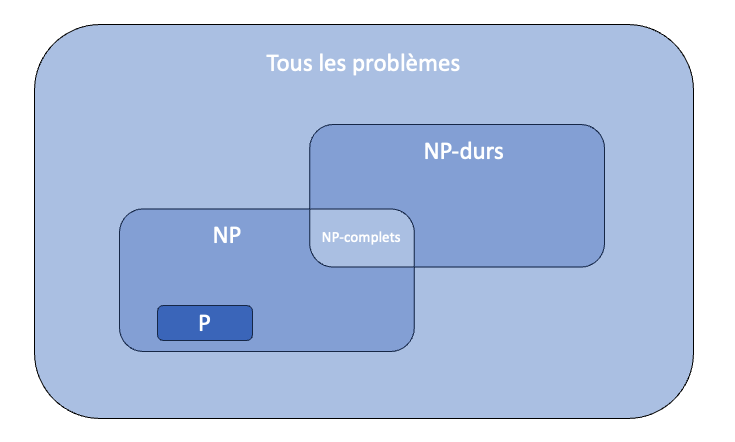
\includegraphics[scale=0.3]{pictures/NP.png}
    \caption{Relations entre les classes de complexité}
\end{figure}
\begin{theorem}{}{} 
    Si $\mathcal{P}\neq\mathcal{NP}$ et un problème $A$ est $\mathcal{NP}$-complet, alors $A\notin \mathcal{P}$.
\end{theorem}
\begin{proof}
    On va supposer que $A\in\mathcal{P}$ et en déduire la contradiction $\mathcal{P}=\mathcal{NP}$. On sait que $\mathcal{P}
    \subseteq\mathcal{NP}$, il nous reste à démontrer que $\mathcal{NP}\subseteq\mathcal{P}$. Soit $B$ un problème de 
    $\mathcal{NP}$ quelconque, montrons qu'il est dans $\mathcal{P}$. \\
    Comme $A$ est $\mathcal{NP}$-complet, $B$ se réduit à $A$ en temps polynomial. Comme $A\in\mathcal{P}$, nous avons un 
    algorithme en temps polynomial pour résoudre $B$ :
    \begin{itemize}[label=\textbullet]
        \item ENTRÉE : Instance $I$ de $B$
        \begin{enumerate}
            \item Transformer $I$ en une instance $I'$ de $A$ en temps polynomial. \textcolor{green}{$O(n^c)$}
            \item Résoudre $I'$ en temps polynomial. \textcolor{green}{$O(n^d)$}
        \end{enumerate}
    \end{itemize}
    Supposons que la réduction se fasse en temps $O(n^c)$ pour une constante $c$ et que $A$ se résout en temps $O(n^d)$ pour
    une constante $d$. Alors $B$ se résout en temps $O(n^{cd})$ :
    \begin{enumerate}
        \item Puisque l'étape 1 se fait en temps $O(n^c)$, où $n$ est la taille de $I$, la taille de $I'$ est en $O(n^c)$.
        \item L'étape 2 est appliquée sur une entrée de taille $O(n^c)$, donc elle prend un temps $O((n^c)^d) = O(n^{cd})$.
    \end{enumerate}
\end{proof}
\begin{lemma}{}{}
    Si vous prouvez qu'un problème $A$ est dans $\mathcal{P}$ et est $\mathcal{NP}$-complet, soit vous avez démontré 
    $\mathcal{P}=\mathcal{NP}$, soit vous avez fait une erreur.
\end{lemma}
\begin{lemma}{}{}
    Si vous ne trouvez pas d'algorithme en temps polynomial pour votre problème, alors peut-être qu'il est $\mathcal{NP}$-complet.
    et dans ce cas vous avez peu de chances d'en trouver un.
\end{lemma}

\subsection{Réduction de SAT vers 3-SAT}